\documentclass{article}
\usepackage{graphicx} % Required for inserting images
\usepackage{url}
\usepackage{hyperref}
\usepackage{verbatim}
\usepackage{natbib}
\usepackage{amsmath} 

\usepackage[letterpaper,top=3cm,bottom=3cm,left=4cm,right=4cm,marginparwidth=1.75cm]{geometry}

\begin{document}

\title{Higher Education Access Disparities in Portugal}
\author{Miguel Sousa Duarte\thanks{{\tiny{}Department of Economics, Copenhagen Business School. \textbf{E-mail}: \url{msd.eco@cbs.dk}.}},
Vicente Conde Mendes\thanks{{\tiny{}École Polytechnique Fédérale de Lausanne. \textbf{E-mail}: \url{vicente.c.mendes@gmail.com}.}}\\}

\date{\today}


\setlength{\parskip}{1em}
\maketitle

\section{Introduction}

Private high-school (HS) students score higher both in internal grading and, most importantly, in National Exams (NE) when compared to public HS students. Either their innate ability is better, or the education provided by private schools is better. In any case, private HS students are certainly privileged. 

Private schools' students score, on average, 4.1 points below on their national exams compared to their school-given grade. For public schools, this gap is of 3.7 points. In fact, as stated by \cite{sapo2024}, the ten 10 HS with the greater difference between internal grading and NE grade are private.
If national exams are a good measure of true ability, then private schools inflate their students' grades by 10\% than public schools. This provides an unfair advantage to private HS students.

\begin{figure}[ht]
  \centering
  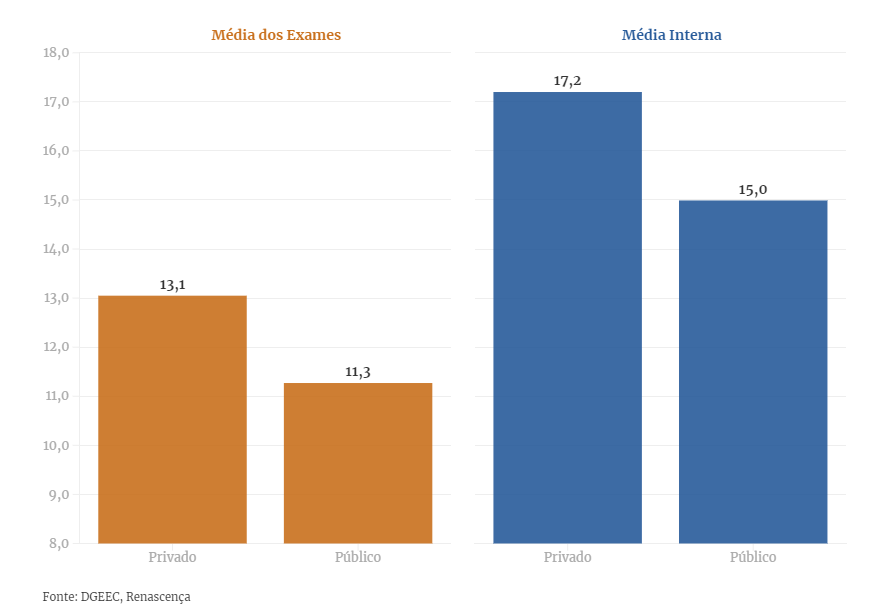
\includegraphics[height=3.5cm, keepaspectratio]{Figures/InflationBySchoolType.png}
  \caption{Inflation by school type}
  \label{fig: InflationBySchoolType}
\end{figure}

\section{Literature Review}

\cite{nata2014unfairness} find that independent private schools inflate their students’ scores when compared to both public and government-dependent private schools. The authors further find that inflation is higher where scores matter most: in the competition for the scarce places available in public higher education. The authors provide descriptive statistics of the grade inflation, without laying out but a small intuition into the implications for access to higher education. We propose an empirical exercise through which the process of accessing higher education is recalculated.

\section{Public University Application Process}


The assignment of students to a certain programme is deterministic in the sense that is exclusively depends on the GPA with which the student concluded High School. 

In Denmark, there is quota 1 and quota 2. Under quota 1, students' probability of getting into a programme is solely dictated by the GPA (henceforth, assume GPA to refer to that of High School graduation). Under quota 2, other factors like sports at a competitive level, internships, motivation, etc. are also taken into account.

There are, nonetheless, a couple differences between the Portuguese system and that of Denmark's quota 1 system. Firstly, in Portugal, the application grade is often composed by 50\% of school-given internal grade and 50\% of national exams relevant for the BSc programme. Two points to note: in Denmark, there are no bachelors-specific exams, in the sense that your GPA is the same regardless of the programme you apply to. (Evidently, you must have taken Mathematics at the A level to study a Bachelors in Economics.) The second one is that, the Portuguese system, by giving greater weight to national exams, already reduces some of the problem that is here under consideration: inflation of school-attributed grade.
Secondly, in Denmark, there is a draw on which national exams one must take, whereas in Portugal, exams are mandatory in the field of HS study, with the students being able to voluntarily sign up for additional exams.


Application grade is often composed by 50\% of school-given internal grade and 50\% of national exams relevant for the BSc programme. National exams are provided and graded by the central government. The exact proportion and which national exams are relevant is defined by the university.
Note that final internal grade is also dependent on national exams. By government rule, for each subject, the internal grade is 70\% teacher's grade and 30\% national exam grade. You can visualize the rules for GPA computation in Figure \ref{fig: GradeComputationPortugal}.

\begin{figure}[ht]
  \centering
  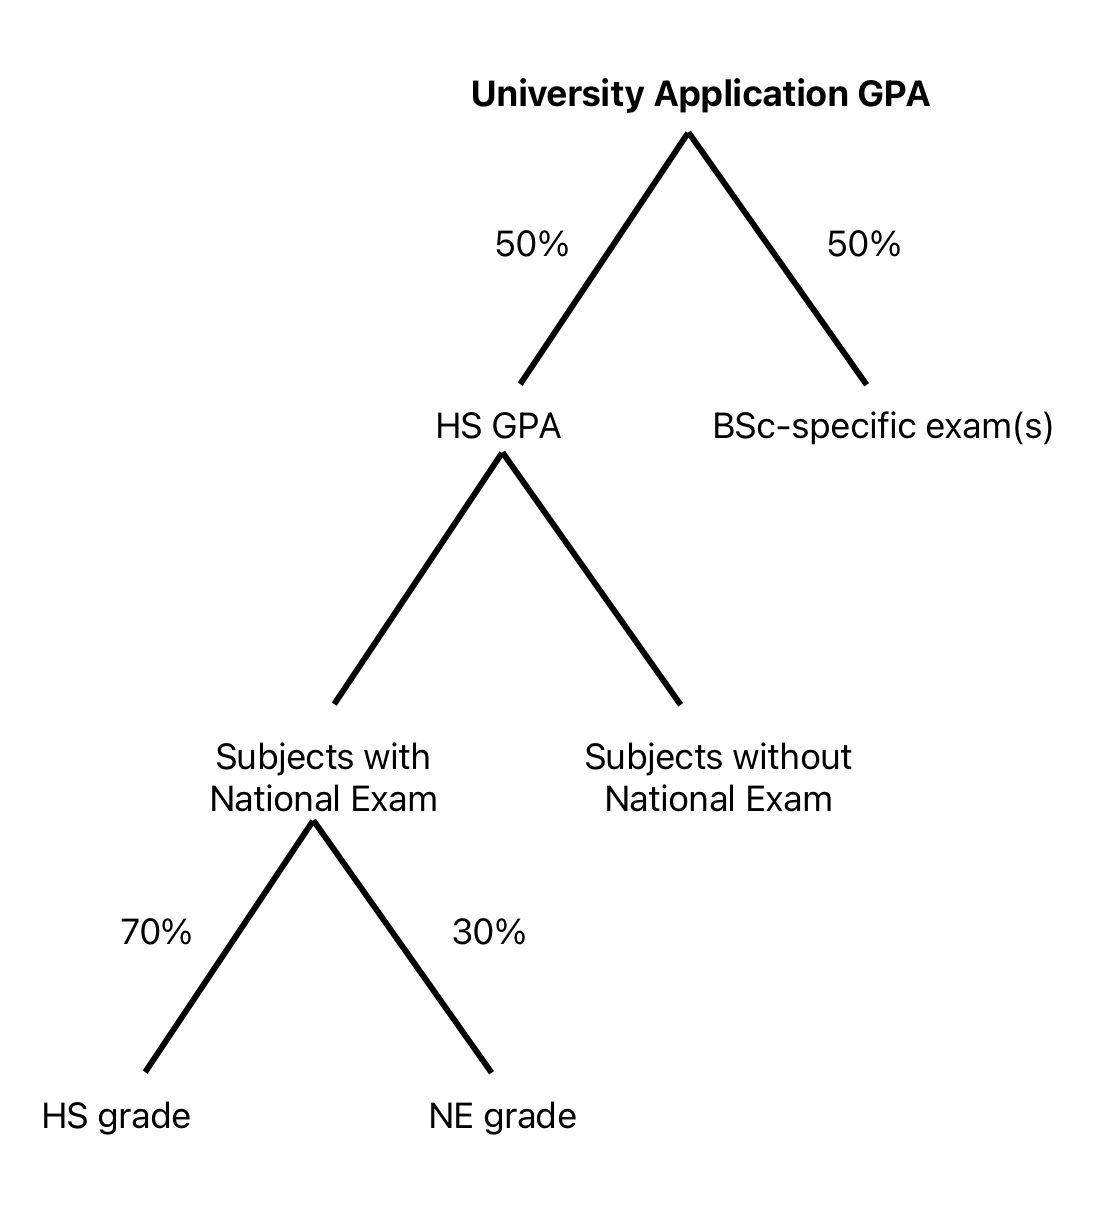
\includegraphics[height=10cm, keepaspectratio]{Figures/GradeComputationPortugal.jpeg}
  \caption{GPA Computation Rules in Portugal}
  \label{fig: GradeComputationPortugal}
\end{figure}


The students rank their 6 programmes of choice when applying to university.

The key factor here is that the schools' internal grading play a relevant role in university application GPA, in a system in which this is the only qualifying mechanism.

\section{Empirical Work}

The first exercise we propose doing is that of taking into account the school-specific grade inflation and performing a simple re-calculation of the assignment of high school graduates to Bachelor programmes. Note that in this first experiment, we implicitly assume that individual's true ability is perfectly represented by the grade scored in the national exam. 
We later relax this assumption. %hopefully

For each subject that is subject to a national exam, find the average grade inflation per school. With individual-level data, re-compute the final grade with which the student applies to university.  

\[
\text{Adj.Grade} = \text{Internal Grade} - \text{Subject School Specific Grade Inflation}
\]  

The Adjusted Final Internal Grade is then computed by using the Adjusted Grades from the subjects in which the student was subject to an exam, together with the original internal ones for subjects the student did not sit for in a national exam.  

The question we want to answer with this re-calculation is the following: Does the proportion of public high school students in high grade requirement courses increase upon this adjustment?

Jacob Østdal suggestion: See two individuals above the cutoff, see one public and private. If private grades are inflated, then the public school kid should have higher ability and do better at university.

\section{Data}
Our data is from the Directorate-General for Statistics of Education and Science (DGEEC) which has data on HS grades, internal and national exams. The choices of HS graduates for public Higher Education are provided by Concurso Nacional de Acesso (CNA) and accessed via DGEEC as well.

What would make the dataset really rich would be to have labour market outcome data that is connected to the DGEEC microdata. To the best of our knowledge, no one has done this before for Portuguese data.

Should we restrict the analysis to Lisbon and Porto?

"In 2009/2010, 76 \% of the students in upper secondary schooling were enrolled in
public institutions (72 \% in ‘regular’ public schools, 4 \% in TEIP schools) and 24 \% in
private schools (19 \% in independent schools, 5 \% in government-dependent private
schools; OECD 2012, p. 333; MEC 2012). The following year, 77 \% of the 377,389 higher
education students were enrolled in public institutions, and the remaining 23 \% in private
ones (Fonseca and Encarnac¸a˜o 2012)."

\section{Empirical Work Summarized}
\begin{itemize}
    \item Assuming national exam performance to be true ability, how does the allocation of Higher Education (HE) slots change if grade inflation is accounted for?
    \begin{itemize}
        \item Do public HS students become better off?
    \end{itemize}
\end{itemize}

Policy changes:

\begin{itemize}
    \item Physical Education recently became part of the HS GPA. There is no reason to believe that private HS are more prone to physical activity, yet %need to back this with data
    they are awarded, on average, higher scores than students in public HS. What was the impact of the change in this policy? How much worse are public HS students?
    \item In the Covid period, rules regarding mandatory NE became more lenient: students only had to take exams used for access to Higher Education. Did teachers inflate grades further given no NE grade to compare the students' school performance to?
\end{itemize}

\section{Empirical Work Done}
We take the grade obtained after the exam, and possible revisions of the grade. We abstract from the fact that there may be a tendency for either public or private HS students to be more likely to ask for a revision of their grade. Given that, when asking for a revision, the student risks ending up with a lower grade than originally, we find this to be a fair assumption.

We start by constructing a variable that we call Inflation which is the result of subtracting the internal grade awarded by the school's teachers by the grade achieved in the exam.

There is something to note here. Internal grading (CIF) is on a scale of 0-20, where as national exam grade (CLASS\_EXAM) is on a scale of 0-200. They are easily comparable and additive if we multiply the former by factor 10. The main thing to note, however, is that the exam grade is more discrete and allows for more differentiation than internal grading.

\cite{nata2014unfairness} divide schools into four different types. We opt for a more parsimonious division and focus only on public and private schools. Inspired by the authors of that paper, we group students by the 1-grade range grade that they scored on the NE, and then plot for each group the mean of the inflation. The plot is brought to you on Figure \ref{fig: Inflation_Nata}

\begin{figure}[ht]
  \centering
  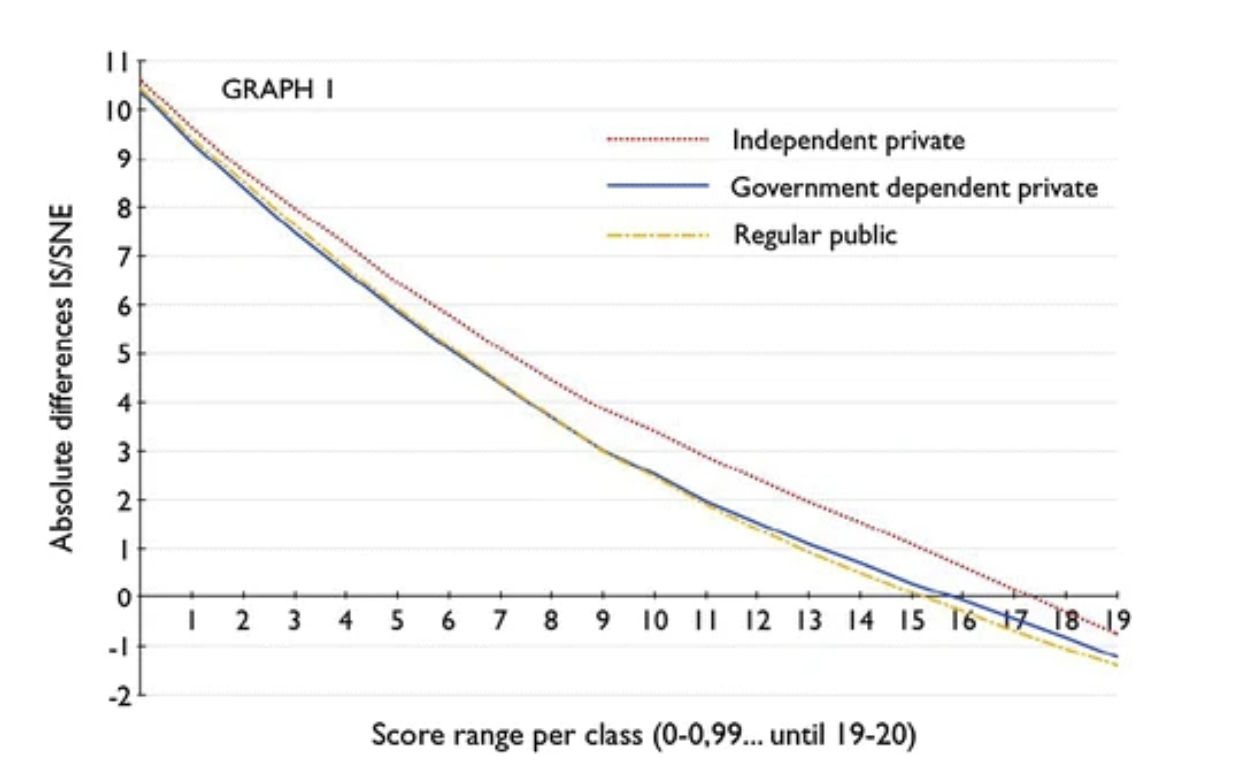
\includegraphics[height=8cm, keepaspectratio]{Figures/Inflation_Nata.png}
  \caption{Inflation plotted against NE grade}
  \label{fig: Inflation_Nata}
\end{figure}

It is clear that for each class of score on NE, the private HS always have a greater differential. This is indicative of some inflation performed by private schools. We explore further this. 
In particular we are interested in understanding the degree of recidivism of schools: are there some schools that consistently exhibit a pattern of higher differential?
We explore the distribution of these differentials, within private and public schools. We see that the across private HS, the variance of differential is much higher than across public schools. The means are not very different in the end, however, there are a few bad boys on the private HS's team that damage the reputation of the overall group.
Narrowing down the bad boys, allows us to see that private HS in the North, particularly in the Porto area, have a greater tendency to have higher differentials than those in the capital Lisbon. Portugal has a centralized government and the exams are put together in Lisbon. We have, however, no reason to believe that this, or any logistics reason, should benefit students in Lisbon.






\section{Extensions}

The inspiration for this section lies on the statement of \cite{nata2014unfairness} that it seems reasonable to assume that grade inflation might be even higher where no comparative scrutiny can be effectively carried out.

Some subjects, like Physical Education (PE) and senior year electives, are not subject to exams yet count for the internal grade. What's more, the data shows that private schools award higher grades on these subjects. How to adjust for this? Physical Education only recently became part of the internal grade, so one can study the impact of its introduction.
\begin{itemize}
    \item I can imagine that top students in public HS still get very nice grades in PE, but maybe the median students in public are worse off than those in private.
\end{itemize}

During the Covid period, exams were easier, graded out of 20 but with 20+ possible points. There were fewer exams, with students only sitting in if needed for university applications, which gave greater relevance to internal grades.

\section{Takeaways}
Public and private high schools differ in many aspects. The investment made per student is not one of them: in fact, the average expense of the Portuguese government with each student is similar, if not higher, to the average private school tuition. However, parents choosing to have their kids go to private school are on average wealthier and more concerned about education. Self-selection in terms of natural ability is likely less explanatory. If your child is not so gifted you might go the extra length to afford a (arguably) better education in the private sector.

In Portugal, there are two perceptions that are seemingly in conflict but may help explain some of the data patterns. The first one is the core issue of this work: grade inflation in the private schools. It is hard to argue that it does not, at least to some extent, occur. The other one is that, it is also not uncommon to hear someone stating that they left private school to go to public school for better grades. Unfortunately or not, private school students are widely accepted to on average be more capable than public school students: if nothing else, from the correlation between wealth and ability. It may then be the case that an above-average student in a private school will come out as a top student in a public school upon moving there.

Using our measure of inflation, we observe that the average inflation across public schools and private schools is not very different. Furthermore, we see a bigger dispersion in the distribution of private schools' inflation. On the one hand, there are some private HS that are well-behaved and inflate as little, if not less, as the public schools inflating the least. On the other hand, the private HS that inflate the most, are also the biggest inflaters from the overall school population: the top 10 inflating schools are all private \citep{sapo2024}.

Our reading is that the well-behaved private schools actually have top students who perform well and lead to low inflations. Also, note that very good students are capped in their inflations by the internal grade upper bound of 20. As for the public schools, these schools have a more concentrated grade inflation. They end up having a lot of low ability students that manage to get a pass in the school grade and then perform poorly in the exam, driving up the inflation for their school. With this in mind, we focus on the students that had internal grading of 14 to 20. Another motivating factor is that these are more likely to be competing for the top spots in public universities.
Finally, we have the misbehaving private schools which are the ones justifying this work. They drive the average of the private inflation up and likely contain the students that made the most advantage of the system, which may have ultimately resulted in taking away public university spots from more deserving public HS students.

Let us think about it as three groups in ascending order of grade inflation: well-behaved private, public and misbehaving private. Well-behaved private HS students achieve top grades in both internal assessment and national exam and therefore go to the top spots. Average public school individuals even with a bigger differential between internal and national exam grading, do not take away university spots from well-behaved private school students. As for the misbehaving private, they do take away university spots from the public HS students, because their high internal grading is driving up their students university application GPA and allowing them to get in front of equally able public HS students.






\newpage
%\bibliographystyle{plainnat}
\bibliographystyle{apalike}
\bibliography{references}

\end{document}